\subsection{Triple Integrals in Cylindrical Coordinates}

\content{
\begin{example} Identify the surface whose equation is 
$$ r=2\sin\theta. $$
\end{example}
}{% presentation
        \vspace{4in}
}{% nopresentation
        \vspace{3in}
}{% comments
}

\content{
}{% presentation
\begin{minipage}{0.3\textwidth}
\begin{example} 
        Set up a triple integral to find the volume of the given shape: \\
        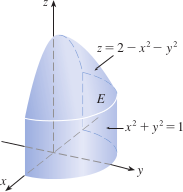
\includegraphics{img/25-1.png}
\end{example}
\end{minipage}
\hspace{1in}
\begin{minipage}{0.3\textwidth}
\begin{example} 
        Set up a triple integral to find the volume of the given shape: \\
        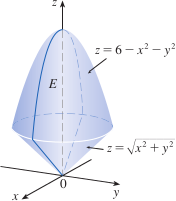
\includegraphics{img/25-2.png}
\end{example}
\end{minipage}
}{ % nopresentation
\begin{example} 
        Set up a triple integral to find the volume of the given shape: \\
        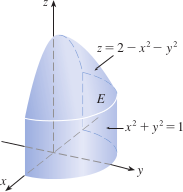
\includegraphics{img/25-1.png}
\end{example}
\vspace{3in}
\begin{example} 
        Set up a triple integral to find the volume of the given shape: \\
        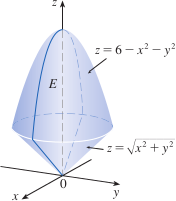
\includegraphics{img/25-2.png}
\end{example}
\vspace{2in}
}{% comments
}

\content{
\begin{example} Evaluate the integral $\iiint_E x^2+y^2\, dV$ where \\
$E = \{(x,y,z) : -2\leq x\leq 2, -\sqrt{4-x^2}\leq y\leq \sqrt{4-x^2}, 
\sqrt{x^2+y^2}\leq z\leq 2\}$.
\end{example}
}{% presentation
}{% nopresentation
        \newpage
}{% comments
}

\content{
\begin{example} Find the volume of the solid which lies above the $xy$-plane and
below the surface $z=4-x^2-y^2$.
\end{example}
}{% presentation
}{% nopresentation
        \vspace{3in}
}{% comments
}

\content{
\begin{example} Evaluate the integral $\iiint_E x\,dV$ where 
$E$ is enclosed by by the paraboloid $x=y^2+z^2$ and the plane $x=4$.
\end{example}
}{% presentation
}{% nopresentation
        \vspace{3in}
}{% comments
}


\content{
\begin{example} Find the volume of the region bounded between the surfaces 
$z=\sqrt{x^2+y^2}$ and $z=6-x^2-y^2$.
\end{example}
}{% presentation
}{% nopresentation
        \vspace{3in}
}{% comments
}
